\chapter{Methodology} \sloppy
\section{Software Development Approach}
 Agile is an iterative process-based approach to software development. In the Agile process model, work is broken down into more manageable, smaller iterations without requiring a lot of long-term planning. The requirements and scope of the project are determined early on, and the number, length, and scope of each iteration are preplanned. Each iteration is considered as a short time ``frame'' in the Agile process model, which lasts for a few weeks. In each iteration, teams move through the phases of the software development life cycle, which include planning, requirements analysis, design, coding, testing, and demonstration of a working product for client review. Agile places a significant value on flexibility, teamwork, and regular client feedback.\\
\begin{figure}[H]
    \centering
    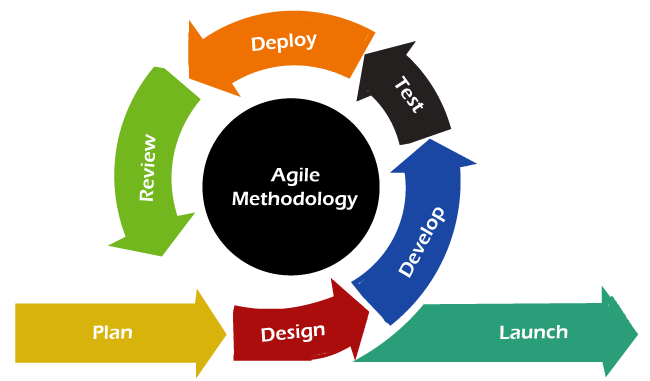
\includegraphics[width=80mm]{./img/agile.png}
    \caption*{\small{\textit{Source: https://www.javatpoint.com/agile-vs-waterfall-model}}}
    \caption{Agile Model}
\end{figure}
The main reason for which  we choose this development process:
\begin{enumerate}[noitemsep] %label=\Roman*.]
\item Very quick,flexible and efficient.
\item Risk minimization.
\item Projects are split into sprints for better management and productivity.
\item Through iterative testing and sprints, the final product contains less bugs. 
\item Development period for application is reduced.
\end{enumerate}
\section{Data Collection} 
We will utilize the IStego100K dataset\cite{7}, a Large-scale open-source image \mbox{steganalysis} dataset. This dataset consits of total 200,000 images, serving as the primary resource for training and testing our model. Within the dataset, images are categorized into two main groups: ``Stego'' and ``Cover,'' each containing 100,000 \mbox{images}. The ``Stego'' subset contains images with hidden information added using three \mbox{different} methods. In contrast, the ``Cover'' subset consists of images without any hidden \mbox{information} added; they are in their original, unaltered state.

\section{Ensemble Classifiers}
Ensemble classifiers are machine learning techniques that combine multiple individual models, or ``base learners,'' to make predictions. Common ensemble techniques include bagging, boosting, and stacking. The main idea behind the ensemble methodology is to weigh several individual classifiers, and combine them in order to obtain a classifier that outperforms every one of them. A standard ensemble approach used in classification tasks consists of the following fundamental components:
\begin{enumerate}
    \item \textbf{Training set:} A labeled dataset used for ensemble training. The training set can be
    described in a variety of languages. Most frequently, the instances are described as attribute-
    value vectors.
    \item \textbf{Base Inducer:} The inducer is an induction algorithm that obtains a training set and
    forms a classifier that represents the generalized relationship between the input attributes
    and the target attribute. Decision trees, Neural networks, Support Vector Machines(SVMs), k-Nearrest Neighbors(k-NN), Random Forsets, Gradient Boosting Machines(GBMs), (AdaBoost) etc. are different types of base learners that can be used in ensemble methods.
    \item \textbf{Diversity Generator:} This component is responsible for generating the diverse
    classifiers.
    \item \textbf{Combiner:} The combiner is responsible for combining the classifications of the various
    classifiers. Some of the widely used combination method are: Weighting method, Majority voting, Performance weighting, Distribution summation, Bayesian combinaiton, Dempster-Shafter, Vogging, Naive bayes.\cite{21} 
\end{enumerate}
\begin{figure}[H]
    \centering
    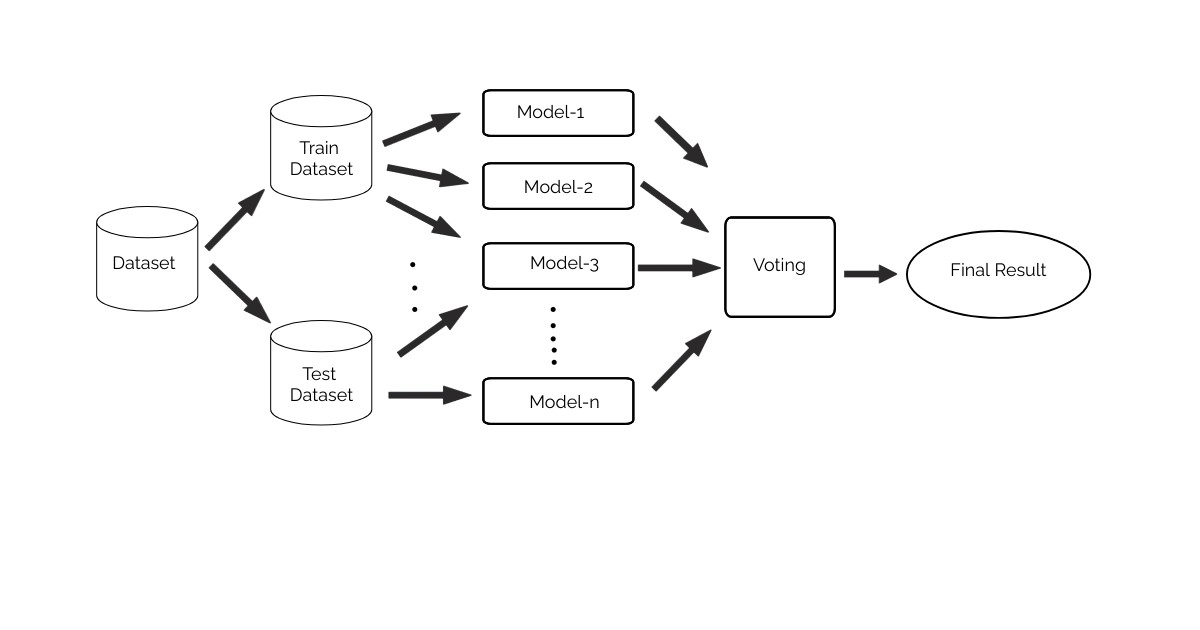
\includegraphics[width=160mm]{./img/ensemble.jpg}
    \caption{Basic outline of Ensemble Classifier}
\end{figure}

\subsection{Algorithm}
\begin{algorithm}
    \caption{Ensemble Classifier Algorithm}
    \begin{algorithmic}[1]
    \For{$l=1$ to $L$}
        \State Form a random subspace
        \State $D_l \subset \{1, \dots, d\}, \lvert D_l \rvert = d_{\text{sub}} < d$
        \State Form a bootstrap sample $N_1^b$, $\lvert N_1^b \rvert = N^{\text{trn}}$ by uniform sampling with \mbox{replacement} from the set $\{1, \dots, N^{\text{trn}}\}$
        \State Train a base learner $B_l$ on features
        \State $X_l = \{x_m^{(D_l)}, \bar{x}_m^{(D_l)}\}_{m \in N_l^b}$
        \State $\rightarrow$ obtain eigenvector $v_l$ and threshold $T_l$
    \EndFor
    \ForAll{$y \in Y^{\text{tst}}$}
        \For{$l=1$ to $L$}
            \State Make $l^{th}$ decision: $B_l(y^{D_l}) \triangleq \begin{cases} 1, & \text{when } v_l^Ty^{(D_l)} > T_l \\ 0, & \text{otherwise} \end{cases}$
        \EndFor
    \EndFor
    \State Form the final decisions $B(y)$ by majority voting: \\
    $B(y) = \begin{cases} 1, & \text{when } \sum_{l=1}^{L} B_l(y^{(D_l)}) > L/2 \\ 0, & \text{when } \sum_{l=1}^{L} B_l(y^{(D_l)}) < L/2 \end{cases}$
    \State \textbf{return} $B(y)$, $y \in Y^{\text{tst}}$
    \end{algorithmic}
    \end{algorithm}
    \clearpage 
    \begin{flushleft}
    In the provided algorithm:\\
    \end{flushleft}
     $d$: Represents the dimensionality of the feature space.\\
     $d_{\text{sub}}$: Represents the dimensionality of the feature subset.\\
     $N^{\text{TRN}}$ and $N^{\text{TST}}$: Denote the number of training and testing examples, respectively.\\
     $L$: Represents the number of base learners.\\
     $x_m, \bar{x}_m \in \mathbb{R}^d, m=1,...,N^{\text{TRN}}$: Refer to the cover and stego features computed from the training set.\\
     $y_k, \bar{y}_k \in \mathbb{R}^d, k=1,...,N^{\text{TST}}$: Denote the cover and stego features computed from the testing set.\cite{5}\\

\section{Implementation}
We start by creating high-dimensional prefeatures that captures various dependencies of the cover elements. We aim to capture as many connections among these elements as we can. For that we will be using CC-C300 model\cite{8} for prefeature extraction. Now, these prefeatures are feeded into an Ensemble based classifier with Fisher Liner Discrimants(FLDs) as the base learners. Random subspace is creating using Bootstrapping and they are given as input to individual base learners. To finalze the final result majority voting is done and final ouput is received. The model is trained several times on IStego100K dataset so that it can predit stego images with high accuracy. 
\begin{figure}[H]
\section{Block diagram of proposed system}
 \centering
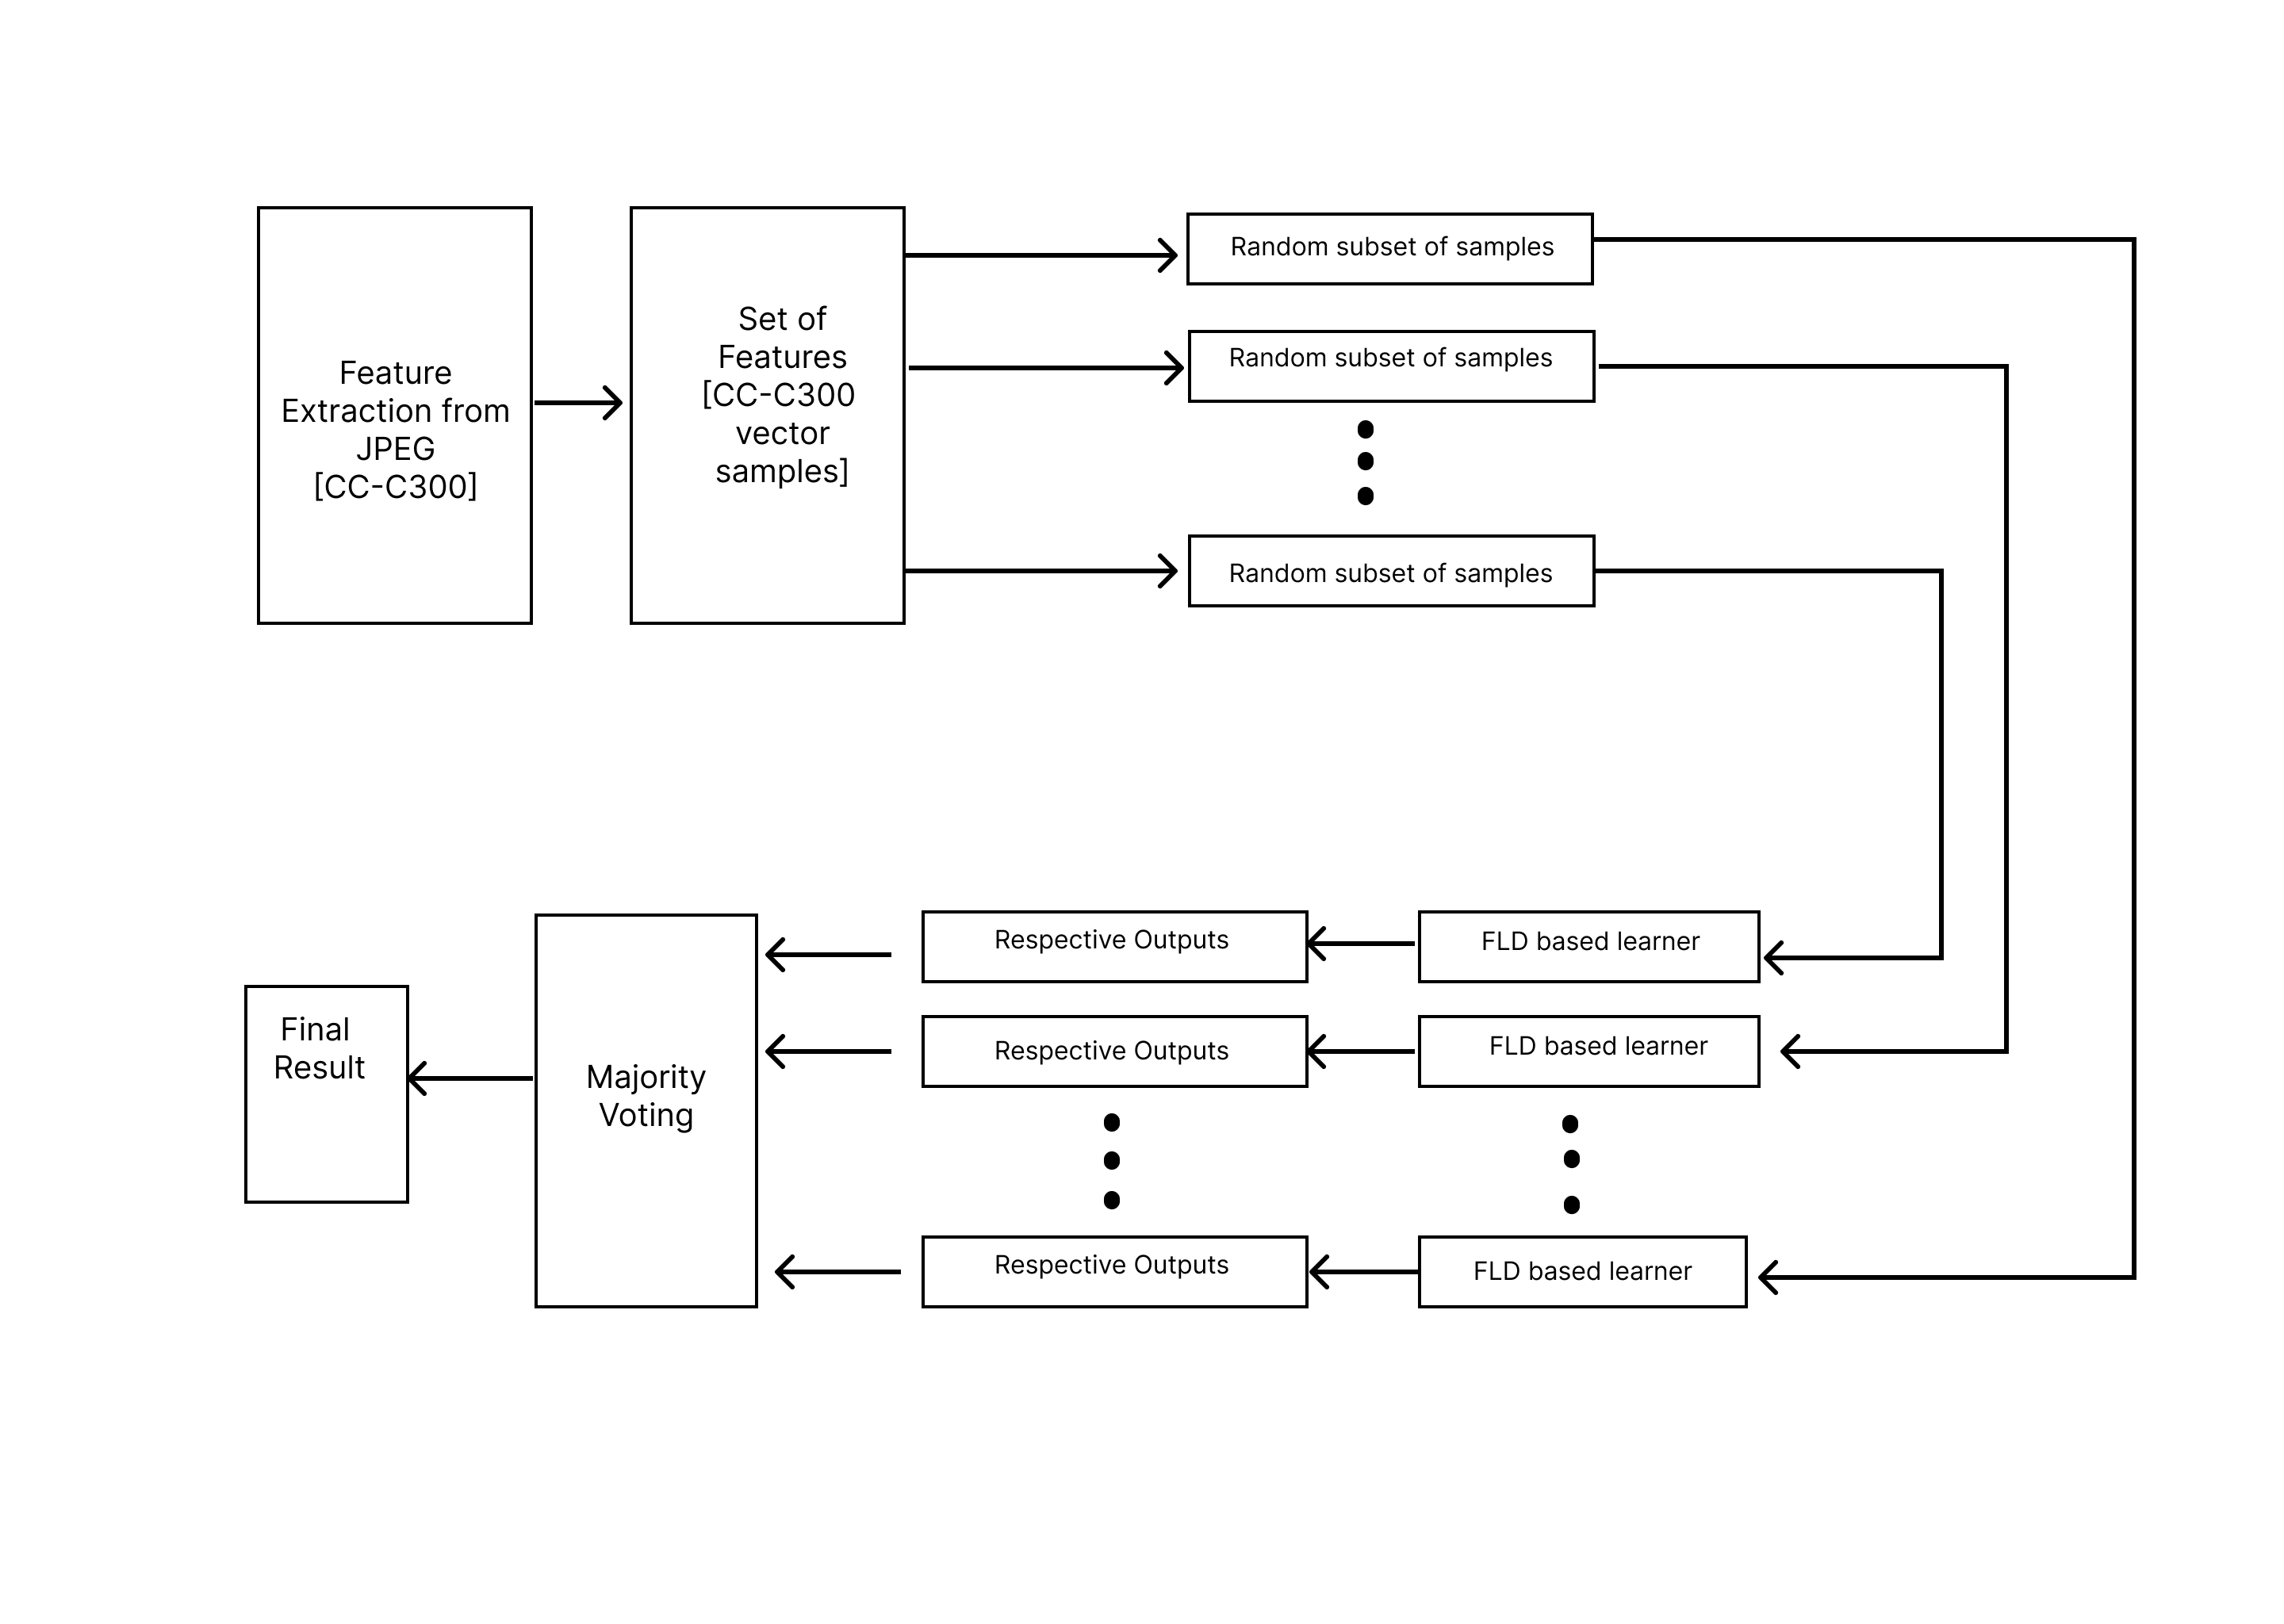
\includegraphics[width=140mm]{./img/model.png}\\
\caption{ Block diagram of proposed system}
\end{figure}
\clearpage

\begin{flushleft}
    \Large{\textbf{Model Training Approach}}\\
\end{flushleft}
\textbf{Feature Extraction:}\\
Initial extraction of CC-C300 feature vector JPEG image is to be done. The selection of CC-C300 is based on its high dimensionality and  its detection efficiency.\vspace{0.25cm}\\
\textbf{Ensemble Classifier Selection:}\\
The decision to choose ensemble classifiers over deep learning techniques was made due to their superior steganalysis detection efficiency and their need for lesser computational power.\vspace{0.25cm}\\
\textbf{Bootstrapping:}\\
Bootstrapping is the process of splitting a large dataset into its smaller subsets. The gathered CC-C300 feature vectors are to be split  into more manageable subsets. Utilizing these subsets, individual base models are to be trained independently.\vspace{0.25cm}\\
\textbf{Base Learner Training:}\\
Based on the extracted features, each base learner independently processes its subset of feature vectors and finalizes a decision.\vspace{0.25cm}\\
\textbf{Aggregation:}\\
To create an ensemble decision, the choices made by each individual base learner are aggregated and the final decision is to be made by using a voting system which finalizes the result by figuring out the most popular output.\vspace{0.25cm}\\
\textbf{Efficiency Considerations:}\\
The proposed system prioritizes efficiency by leveraging shallow machine learning techniques, particularly ensemble classifiers instead of deep learning. The choice of CC-C300 as a feature is intentional to increase efficiency and detection capability of the system.\\
\clearpage 

\section{System Architecture}
\begin{figure}[H]
    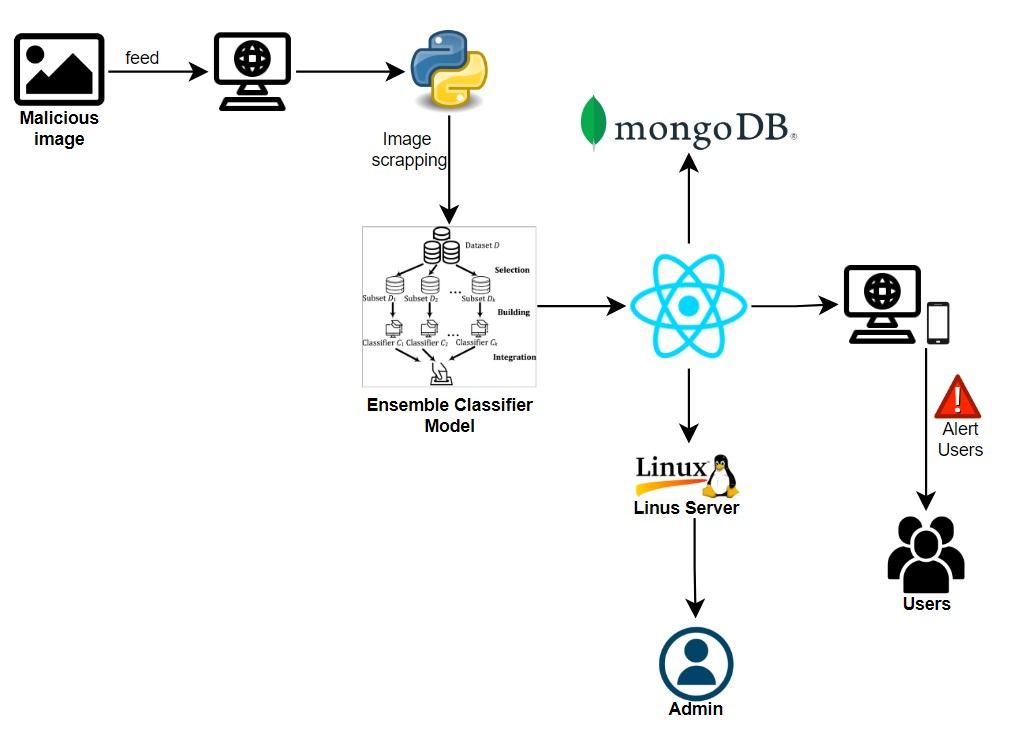
\includegraphics[width=150mm]{./img/System architecture.jpg}
    \caption{System Architecture}
\end{figure}
\clearpage 
